\chapter{Experimental Setting and Results}
% This section provides an overview of the experimental setting used to evaluate Internet Explorer, as well as the key results of our experiments in these settings.
This section provides an overview of the experimental setting used to evaluate Internet Explorer, as well as detailed results and analysis of our experiments in these settings.

\section{Experimental Setting}
\subsection{Self-supervised Exploration}
% explain why this setting is important, and explain the baselines 
To make Internet Explorer as widely applicable as possible, we first evaluate it in a setting where we assume no prior knowledge of the contents of the images 




We assume that we have an unlabeled target dataset of images for which we would like to learn useful visual features. We compare three methods:
% EB: we should consider a better abbreviated method name. how about: IE, IE+?
% \begin{enumerate}[noitemsep,topsep=0pt]
%     \item Random: sample queries uniformly at random from the vocabulary. 
%     \item Ours: sample queries from our learned concept distribution. 
%     \item Ours++: additionally use GPT-generated descriptors
% \end{enumerate}
% \begin{enumerate}[noitemsep,topsep=0pt]
\begin{enumerate}
    \item Random: sample concepts uniformly from the vocab. 
    \item Ours: sample concepts from our learned distribution. 
    \item Ours++: additionally use GPT-generated descriptors.
\end{enumerate}
% lack of label knowlege makes this challenging but also generally applicable
% This setting is challenging because we have to explore to discover what concepts are useful for our target dataset, without any prior knowledge of what those concepts might be. 
The lack of label knowledge makes this setting challenging, but also very general. Our method is forced to explore the space of concepts to discover what is useful for the target dataset, without any prior knowledge of what might be useful.

\begin{figure*}[t]
    \centering
    \includegraphics[width=\linewidth]{figures/ssl-curves-updated.pdf}
    \caption{\textbf{Learning curves in self-supervised setting.} $k$-NN validation accuracy improves across iterations on each target dataset. Without using any labels, Internet Explorer identifies and focuses on relevant concepts for each target dataset. This allows it to find more useful data than the baseline that searches for random concepts. Adding GPT-generated descriptors (Ours++) further improves performance by enabling Internet Explorer to generate diverse views of useful concepts. 
    % Interestingly, the random baseline does quite well on VOC2007, perhaps because coarse-grained classification benefits from a broader variety of training data. 
    } 
    \label{fig:learning_curves}
\end{figure*}

\begin{figure*}[t]
    \centering
    \includegraphics[width=\linewidth]{figures/semisup-curves-updated.pdf}
    \vspace{-0.3in}
    \caption{\textbf{Learning curves in label set-guided setting.} Using knowledge of the label set improves the performance of all methods. Internet Explorer (Ours) outperforms the baselines on all datasets, and adding GPT-generated descriptors (Ours++) further improves performance.
    }
    \label{fig:semisup_learning_curves}
    % \vspace{-0.05in}
\end{figure*}


\subsection{Label Set-guided Exploration}
% explain why this setting is also potentially practical 
% explain the baselines 
In practice, we may sometimes know the set of labels for our task even if we do not have image-label pairs (\ie, the English names of the classes).
For example, we may know that our data contains images of ``Golden Retrievers,'' ``Maine Coon,'' \etc, even if we do not have any images labeled with these names.
Knowing the label set greatly accelerates learning on the Internet, because it acts as a strong prior on what could be useful for our target dataset and allows us to focus our exploration on the subset of the vocabulary that is most likely to be useful.
Using our text similarity model, we reduce the size of the vocabulary by selecting the top 
% 10,000 concepts
$10\%$ ($14{,}635$ concepts)
with the largest average top-$k$ similarity to the label set in text embedding space. We set $k$ to a third of the size of the label set to reduce the impact of outliers.
Restricting our vocabulary to a semantically relevant subset also strengthens our baselines by ensuring that they only search for potentially useful concepts.

We compare 4 methods in this setting:
\begin{enumerate}[noitemsep,topsep=0pt]
    \item Labels: only search for labels. 
    \item Labels + relevant: search for labels half of the time, and random concepts from the pruned vocabulary the other half of the time. 
    \item Ours: sample labels half of the time and sample from our learned concept distribution the other half. 
    \item Ours++: additionally use GPT-generated descriptors.
\end{enumerate}
We call this setting ``label set-guided,'' since we have additional supervision in the form of the label set.

% \subsection{Datasets and Metrics}
\subsection{Datasets}
We evaluate Internet Explorer on 4 popular small-scale fine-grained classification datasets: Birdsnap~\cite{berg2014birdsnap}, Flowers-102~\cite{nilsback2008automated}, Food101~\cite{bossard2014food}, and Oxford-IIT Pets~\cite{parkhi2012cats}.
% which are commonly used to evaluate transfer learning for large pre-trained models~\cite{kornblith2019better}. 
We also evaluate on Pascal VOC 2007 (Classification)~\cite{everingham2010pascal}---a coarse-grained multi-label classification task consisting of only $2{,}040$ training examples, making it ideal for testing whether Internet Explorer can efficiently find relevant useful data.
We do not target large-scale datasets like ImageNet~\cite{deng2009imagenet} because they already contain over a million human-curated Internet images.
% We compare the representation quality of our model \wrt~its target dataset using two metrics: $k$-nearest neighbors ($k$-NN) accuracy and linear probe accuracy. 
% $k$-NN accuracy can be computed quickly, so we use this to plot learning curves of model performance after every iteration during training. We report the early-stopped linear probe accuracy in our tables.

\subsection{Evaluation Metrics}
We compare the representation quality of our models using two metrics: k-nearest neighbors (k-NN) accuracy  and linear probe accuracy. To measure k-NN accuracy, we use our ResNet-50 to encode each dataset's training and test sets. Then, for each test example, we find its $k$ nearest neighbors in representation space and use the mode of its neighbors' labels as the prediction. We use k-NN accuracy to plot learning curves of model performance after every iteration, since it is easy to quickly compute.

To compute the linear probe accuracy, we first select the best-performing model over all iterations on the validation set according to the k-NN accuracy. Then, we learn a linear head on top of these learned representations by minimizing the cross-entropy loss. We tune the weight decay parameter in the logscale range $(10^{-6}, 10^6)$, as is done in~\cite{radford2021learning}, using \texttt{scikit-learn}~\cite{pedregosa2011scikit} with Brent's method~\cite{brent1973algorithms}.


\begin{table}[t]
    \centering
    \begin{adjustbox}{width=1\textwidth}
    \begin{tabular}{lc@{\hskip 0.12em}cc@{\hskip 0.12em}cc@{\hskip 0.12em}cc@{\hskip 0.12em}cc@{\hskip 0.12em}cc@{\hskip 0.12em}cc@{\hskip 0.12em}cc}
    \toprule
        % Model & Flowers102 & Food101 & Stanford Cars & Oxford-IIIT Pets & Total Images & GPU-hours \\
        Model & \multicolumn{2}{l}{Birdsnap} & \multicolumn{2}{l}{Flowers} & \multicolumn{2}{l}{Food}  & \multicolumn{2}{l}{Pets} & \multicolumn{2}{l}{VOC2007} & Images & GPU hrs. \\
    \midrule
    % \textit{Fixed dataset, language supervision} \\
    \textit{Fixed dataset, lang. supervision} \\
        \;\;\;CLIP ResNet-50 (\textbf{oracle})  & $57.1$ & & $96.0$ & & $\bf{86.4}$ & & $88.4$ & & $\bf{86.7}$ & & $400 \times 10^6$ & $4{,}000$ \\ % 82.8 for CLIP pascal 
    \midrule
    \textit{Fixed dataset, self-supervised} \\
        \;\;\;MoCo-v3 (ImageNet pre-train)  & $26.8$ & & $83.2$ & & $70.5$ & & $79.6$ & & $-$ & &  $1.2 \times 10^6$ & $72$ \\
        %\;\;\; MoCo-v3 (target only)                      & 80.0 & 0    & 0    & $< 10^5$ & 2 \\
        \;\;\;MoCo-v3 (ImageNet + target)  & $39.9$ & & $94.6$ & & $78.3$ & & $85.3$ & & $58.0^\dag$ & & $1.2 \times 10^6$ & $72 + 12$ \\
    \midrule
    \textit{No label set information} \\
        \;\;\;Random exploration  & $39.6$ & \red{$(-0.3)$} & $95.3$ & \green{$(+0.7)$} & $77.0$ & \red{$(-1.3)$} &  $85.6$ & \green{$(+0.3)$} & $70.2$ & \green{$(+12.2)$} &  $2.2 \times 10^6$ & $84 + 40$ \\
        \;\;\;Ours  & $43.4$ & \green{$(+3.5)$} & $97.1$ & \green{$(+2.5)$} & $80.5$ & \green{$(+2.2)$} & $86.8$ & \green{$(+1.5)$} & $68.5$ & \green{$(+10.5)$}  & $2.2 \times 10^6$ & $84 + 40$ \\
        \;\;\;Ours++  & $54.4$ & \green{$(+14.5)$} & $98.4$ & \green{$(+3.8)$} & $82.2$ & \green{$(+3.9)$} & $89.6$ & \green{$(+4.3)$} & ${80.1}$ & \green{${(+22.1)}$} & $2.2 \times 10^6$ & $84 + 40$ \\
    \midrule 
    \textit{Use label set information} \\       
        \;\;\;Search labels only  & $47.1$ & \green{$(+7.2)$} & $96.3$ & \green{$(+1.7)$} & $80.9$ & \green{$(+2.6)$} & $85.7$ & \green{$(+0.4)$} & $61.8$ & \green{$(+3.8)$} & $2.2 \times 10^6$ & $84 + 40$ \\
        \;\;\;Labels + relevant terms  & $49.9$ & \green{$(+10.0)$}& $98.0$ & \green{$(+3.4)$} & $81.2$ & \green{$(+2.9)$} & $87.0$ & \green{$(+1.7)$} & $67.5$ & \green{$(+9.5)$} & $2.2 \times 10^6$ & $84 + 40$ \\
        \;\;\;Ours  & $52.0$ & \green{$(+12.1)$} & $97.6$ & \green{$(+3.0)$} & $81.2$ & \green{$(+2.9)$} & $87.3$ & \green{$(+2.0)$} & $70.3$ & \green{$(+14.3)$} & $2.2 \times 10^6$ & $84 + 40$ \\
        \;\;\;Ours++  & $\mathbf{62.8}$ & \green{$\mathbf{(+22.9)}$} & $\bf{99.1}$ & \green{$\mathbf{(+4.5)}$} & $84.6$ & \green{$(+6.3)$} & $\mathbf{90.8}$ & \green{$\mathbf{(+5.5)}$} & ${79.6}$ & \green{$(+21.6)$} & $2.2 \times 10^6$ & $84 + 40$ \\
    \bottomrule
    \end{tabular}
    \end{adjustbox}
    % \caption{\textbf{Linear probe accuracy on targeted datasets}.}
    \caption{\textbf{Linear probing accuracy}. Our method significantly improves the starting checkpoint performance in just 40 additional hours of training. We show the performance change from the starting MoCo-v3 (ImageNet + target) initialization in \green{green}/\red{red}. CLIP numbers correspond to linear probe (which is higher than its zero-shot accuracy). Internet Explorer reaches or often surpasses CLIP (oracle with 2x params) performance on each dataset while using 2.5\% as much compute and 0.5\% as much data. ${}^{\dag}$For VOC2007, we do not do ImageNet pre-training because ImageNet is too close to VOC2007.
    % obscures the effect of Internet Explorer. 
    % We report $k$-NN accuracy in the VOC2007 column and show LP in the supplementary. 
    }
    \label{tab:main_results}
\end{table}


\begin{figure}[t]
\centering
\includegraphics[width=0.675\linewidth]{figures/pets_ssl_reward_over_training2.pdf}
\caption{\textbf{Self-supervised concept discovery on Pets dataset.} When targeting the Pets dataset, self-supervised Internet Explorer quickly estimates high reward for concepts from the cat category (82 concepts) and dog category (246 concepts). It is also able to identify felines that are not cats (e.g., tigers) and canines that are not dogs (e.g., wolves), although it gives them lower reward on average. Finding these categories is especially challenging, since they comprise only $460/146{,}347 = 0.3\%$ of the vocabulary.}
\label{fig:reward_over_training}
\end{figure}



\begin{figure*}[t]
    \centering
    \includegraphics[width=\linewidth]{figures/pets_targets.pdf}\\
    \includegraphics[width=\linewidth]{figures/pets-progression-962-2col-3row.pdf}
    % \includegraphics[width=\linewidth]{figures/pets-progression-962-2col.pdf}
    \caption{
    % \textbf{Progression of downloaded images over training.} The top row shows the target distribution and the bottom ones show the sets of images queried by our Internet Explorer. As the progression goes on, the image set discovered by the Internet Explorer starts to more closely resemble the target dataset distribution.
    \textbf{Progression of downloaded images across training.} \textbf{Top:} samples of Oxford-IIIT Pets images.\ \textbf{Bottom:} samples of images queried by Internet Explorer across iterations. As the method learns, it makes queries that are progressively more relevant to the target dataset.
    }
    \label{fig:progression}
    \vspace{-0.15in}
\end{figure*}

\section{Results and Analysis}
\subsection{Self-supervised Results}
\cref{fig:learning_curves} shows how Internet Explorer improves the $k$-NN accuracy more efficiently than sampling queries uniformly at random from the concept vocabulary. In fact, random sampling occasionally decreases accuracy, likely due to the fact that Internet images can generally be unsuitable for pre-training due to issues such as watermarks, images containing text, and overly photogenic images~\cite{mezuman2012learning,chen2015webly}. \cref{tab:main_results} shows that our method significantly improves on the starting MoCo-v3 (ImageNet + target) checkpoint and can outperform a CLIP~\cite{radford2021learning} model of the same size while using much less compute and data. This is impressive as CLIP can be thought of as an oracle, since its training set contains up to 20k Bing image search results for each WordNet lemma (in addition to other queries).
Using GPT-generated descriptors in ``Ours++'' also significantly improves performance by enabling Internet Explorer to generate diverse views of the most useful concepts. 
% We show example image results with and without descriptors in the supplementary. 

\subsection{Self-supervised Exploration Behavior}
\label{sec:exploration_behavior}
\cref{fig:reward_over_training} shows the progression of Internet Explorer (Ours++) behavior on the Pets dataset in the self-supervised setting. Since Pets consists of cat and dog breeds, to analyze the results, we use the WordNet hierarchy to divide concepts in our vocabulary into 5 meaningful categories: cats, dogs, non-cat felines (e.g., lion), non-dog canines (e.g., wolf), and other. This categorization is only done for this post hoc analysis and is not provided during training. \cref{fig:reward_over_training} (top) shows that
% the average estimated reward within each category across the first 20 iterations of training, and the bottom one shows how much probability mass each category has. 
Internet Explorer rapidly identifies the roughly $0.3\%$ of concepts that are useful for Pets. During the first two iterations, the average estimated reward for each category is roughly the same. However, after the first dog concept is searched in iteration $\#2$, the estimated reward and probability mass for dogs and other canines rapidly increases. The same happens for cats after the first cat is searched in iteration $\#4$. Interestingly, while ``other felines'' and ``other canines''  have higher average reward than the ``other'' category, they still have much lower reward than cats and dogs. This indicates that our model understands that other felines and canines (mostly large, wild predators) are only moderately relevant for house pet cats and dogs. 

\cref{fig:progression} shows how Internet Explorer downloads progressively more useful images over time. It shows 8 random images that were downloaded in iteration $\#0$, $\#1$, $\#3$, $\#6$, $\#10$, and $\#15$. Iteration $\#0$ contains mostly useless data, like graphics or screenshots, but Pets-relevant images already make up most of the downloads by iteration $\#3$. 
Results for other datasets are shown in \cref{sec:progression_continued}.

\subsection{Label Set-guided Results}
% As discussed earlier, we now make use of the label set of the target dataset without knowing the exact image-label mapping. 
Internet Explorer significantly outperforms the stronger baselines in the label set-guided setting where we additionally have knowledge of the label set. Searching for the label set continuously provides useful data and helps us rapidly identify other useful concepts. Together with the diversity promoted by GPT descriptors, Ours++ outperforms CLIP in 3/5 datasets and approaches its performance in the other 2, using just 2.5\% of the time and 0.5\% the data---as can be seen in \cref{tab:main_results}. The fact that Ours++ can match/outperform CLIP is especially impressive, since CLIP has access to up to 20k Bing image search results for each WordNet lemma (in addition to other queries).
k-NN accuracy learning curves for the label set-guided setting are shown in \cref{fig:semisup_learning_curves}.

% Note that we train Internet Explorer from scratch on VOC2007 and do not use an ImageNet pre-trained MoCo-v3 model as initialization. 
% Note that we train from scratch on VOC2007 and do not do ImageNet pre-training because ImageNet's similarity to VOC2007 obscures the effect of Internet Explorer.

\subsection{Learning from other sources of data}
\label{subsec:search_engine_main}

Google Images is an exceptionally useful data source for Internet Explorer. It offers access to a large portion of the Internet's images, and it ranks images using weak supervision from the image caption, surrounding text, click rates, image features, incoming and outgoing hyperlinks, and other signals. This extra supervision is helpful and should be utilized. Nonetheless, we show that Internet Explorer is agnostic to the choice of text-to-image search engine and can still rapidly improve even when the data source is much noisier. 

\begin{table*}[h]
    \centering
    \begin{adjustbox}{width=1\textwidth}
    \begin{tabular}{@{\extracolsep{4pt}}lccccccccc}
    \toprule
        % Model & Flowers102 & Food101 & Stanford Cars & Oxford-IIIT Pets & Total Images & GPU-hours \\
        \multirow{2}{*}{\textbf{Model}}
        &\multicolumn{3}{c}{\textbf{Flowers}} 
        &\multicolumn{3}{c}{\textbf{Food}}
        &\multicolumn{3}{c}{\textbf{Pets}} \\
        \cmidrule{2-4} \cmidrule{5-7} \cmidrule{8-10}
        
        
        & Google & Flickr & LAION & Google & Flickr & LAION & Google & Flickr & LAION \\
    \midrule
    \textit{Fixed dataset} &&&&&&&&&\\    
        \;\;\; MoCo-v3 (IN)                          & $83.2$ & $83.2$ & $83.2$ & $70.5$ & $70.5$ & $70.5$ & $79.6$ & $79.6$ & $79.6$ \\
        \;\;\; MoCo-v3 (IN + target)                 & $94.6$ & $94.6$ & $94.6$ & $78.3$ & $78.3$ & $78.3$ & $85.3$ & $85.3$ & $85.3$ \\
    \midrule
    \textit{Undirected search} &&&&&&&&&\\    
        \;\;\;Random exploration                     &  $95.3$  &  $95.2$  &  $94.8$  &  $77.0$ &  $80.0$  &  $80.2$  &  $85.6$ & $84.4$  & $85.1$ \\
    \midrule 
    \textit{Internet Explorer} &&&&&&&&&\\    
        % \;\;\;Random exploration                      &    &    &    &    &    &    &    &    &    \\
        % \;\;\;Ours                                   &  ? &  ? &  ? &  ? &  ? \\
        \;\;\;Ours++ (no label set)                  &  $98.4$  &  $98.1$  &  $94.6$  &  $81.2$  &  $80.3$  &  $80.9$  &  $87.3$  &  $88.4$  &  $85.9$  \\
    % \midrule 
        % \;\;\;Search labels only                      &  ? &  ? &  ? &  ? &  ? \\
        % \;\;\;Labels + relevant                       &    &    &    &    &    &    &    &    &    \\
        % \;\;\;Ours                                    &  ? &  ? &  ? &  ? &  ? \\
        \;\;\;Ours++ (with label set)                &  $\bf{99.1}$ &  $\bf{99.0}$ &  $\bf{95.8}$ & $\bf{84.6}$ & $\bf{81.9}$  &  $\bf{81.0}$  & $\bf{90.8}$ &  $\bf{89.1}$  &  $\bf{86.7}$  \\
    \bottomrule
    \end{tabular}
    \end{adjustbox}
    \caption{\textbf{Linear probe accuracy with other search engines}. Internet Explorer improves its performance using any search engine, including Flickr and our custom text-based LAION search engine.}
    \label{tab:search_engine}
\end{table*}

\begin{figure*}[p]
    \centering
    \includegraphics{figures/food-spaghetti.pdf} \\
    \includegraphics{figures/google-spaghetti.pdf} \\
    \includegraphics{figures/flickr-spaghetti.pdf} \\
    \includegraphics{figures/laion5b-spaghetti.pdf} 
    \caption{\textbf{Comparison of different search engines.} We show images for the ``spaghetti bolognese'' class in the Food101 dataset, as well as 20 search results for ``spaghetti bolognese'' from Google Images, Flickr, and LAION5B. Google images are typically well-lit, aesthetic food blog pictures. In comparison, Flickr images are messier, darker, and capture a wider variety of real-world conditions. LAION-5B images lie somewhere in the middle, but contain text overlays much more frequently. Duplicate image results are also common.}
    \label{fig:data_comparison}
\end{figure*}

\begin{wrapfigure}{R}{0.4\textwidth}
\centering
    \vspace{-2em}
    \includegraphics[width=\linewidth]{figures/laion_search_engine.pdf}
    \vspace{-1em}
    \caption{\textbf{Custom LAION-5B search engine.} We build a custom text-to-image search engine that finds images within the LAION-5B dataset by doing nearest neighbor search in text embedding space---using no image features whatsoever.}
    \label{fig:laion_search_engine}
    \vspace{-4em}
\end{wrapfigure}

To test Internet Explorer in the most minimal setting, we build a custom search engine that finds images solely using their accompanying text, without using any pre-trained visual features whatsoever. We use the LAION-5B dataset~\cite{schuhmann2022laion}, which consists of 5.85 billion noisy image-caption pairs. We filter the dataset to only include samples with English captions and images with at least $512^2$ pixels. This leaves us with about 600M text-image pairs. To find image results for a query, we find the 100 captions closest to the query in text representation space, then return the associated images.
We use a pre-trained text embedding model~\cite{reimers2019sentence} to compute 384-dimensional text embeddings for each caption. Then, we use Faiss~\cite{johnson2019billion} to compute a fast, approximate nearest-neighbors lookup index. Querying our custom search engine finds 100 image results in less than a second. \cref{fig:laion_search_engine} shows that our search engine is reasonably accurate, even without using any image features. 

We also test Flickr's photo search API as another text-to-image search engine, in addition to Google Images and LAION. \cref{fig:data_comparison} shows that each data source has its own tendencies. For the ``spaghetti bolognese'' query, Google Images is biased~\cite{mezuman2012learning,chen2015webly} towards brightly-lit, photogenic images that typically come from food blogs. Flickr mainly consists of amateur home photos, so it returns a messier variety of images that perhaps better capture the real world. LAION images come from web crawling, without any ranking, so they additionally contain many graphics with text overlays. The same image can also frequently show up in the LAION results multiple times, as a result of being posted on multiple separate pages. 


\begin{figure*}
    \centering
    \includegraphics[width=\linewidth]{figures/laion-curves.pdf}
    \caption{\textbf{Learning from Flickr and LAION-5B.} Even with the noisy search results returned by Flickr and LAION, Internet Explorer still continuously improves performance. }
    \label{fig:other_data_curves}
\end{figure*}


\cref{fig:other_data_curves} and \cref{tab:search_engine} show that Internet Explorer consistently improves over time, regardless of the search engine we use. 
Google consistently does best, followed by Flickr, then LAION (which has the smallest pool of images to draw from).
Using Internet Explorer to search LAION-5B consistently performs \textit{better} than random exploration---indicating that Internet Explorer is effective even for selecting data from a static dataset.
Overall, these results are proof that Internet Explorer can effectively utilize any window into the Internet's vast ocean of image data. 


\subsection{Are we finding the entire test set online?}
\label{sec:finding_test_set_online}

\newcommand{\blue}[1]{\textcolor{Cerulean}{#1}}
\begin{table}[t]
    \centering
    % \begin{tabular}{lccccccccc}
        \begin{adjustbox}{width=1\textwidth}
        \begin{tabular}{
            lr@{\hskip 0.12em}
            rr@{\hskip 0.12em}
            rr@{\hskip 0.12em}
            rr@{\hskip 0.12em}
            rr@{\hskip 0.12em}
            rc}
        \toprule
            % Model & Flowers102 & Food101 & Stanford Cars & Oxford-IIIT Pets & Total Images & GPU-hours \\
            % Model & Birdsnap & Flowers & Food  & Pets & VOC2007  & Images Downloaded \\
            &
            \multicolumn{2}{l}{Birdsnap} & 
            \multicolumn{2}{l}{Flowers} & 
            \multicolumn{2}{l}{Food} & 
            \multicolumn{2}{l}{Pets} & 
            \multicolumn{2}{l}{VOC2007} \\
        \midrule
        Target test set size                          &  \multicolumn{2}{l}{$1849$} &  \multicolumn{2}{l}{$6142$} & \multicolumn{2}{l}{$25246$} &\multicolumn{2}{l}{$3663$} &\multicolumn{2}{l}{$4952$} \\ 
        % Target test set size                          &  \multicolumn{2}{c}{$1849$} &  \multicolumn{2}{c}{$6142$} & \multicolumn{2}{c}{$25246$} &\multicolumn{2}{c}{$3663$} &\multicolumn{2}{c}{$4952$} & $-$ \\ 
        \midrule
        \textit{No exploration} \\
            \;\;\; Target training set overlap                          &  $1$ & \blue{$(0.05\%)$} &  $5$ & \blue{$(0.01\%)$}& $34$ & \blue{$(0.13\%)$} & $21$ & \blue{$(0.57\%)$} &  $0$ & \blue{$(0.00\%)$} \\
        \midrule
        % \textit{No label set information} \\
        \textit{Internet Explorer} \\
            % \;\;\;Random exploration                     &  ? &  ? &  ? &  ? &  ? \\
            % \;\;\;Ours                                   &  ? &  ? &  ? &  ? &  ? \\
            % \;\;\;Ours++ (no label set)                         &  $28/1849$ & & $11/6142$ & & $35/25246$ & & $26/3663$ & & $1/4952$ & & $\approx 10^6$\\
            \;\;\;Ours++ (no label set)                         &  $28$ & \blue{$(+1.46\%)$} & $11$ & \blue{$(+0.01\%)$} & $35$ & \blue{$(+0.00\%)$} & $26$ & \blue{$(+0.14\%)$}& $1$ & \blue{$(+0.02\%)$} \\
        % \midrule 
        % \textit{Use label set information} \\       
            % \;\;\;Search labels only                      &  ? &  ? &  ? &  ? &  ? \\
            % \;\;\;Labels + semantically relevant terms    &  ? &  ? &  ? &  ? &  ? \\
            % \;\;\;Ours                                    &  ? &  ? &  ? &  ? &  ? \\
            \;\;\;Ours++ (with label set)                       & $57$ & \blue{$(+3.03\%)$} & $27$ & \blue{$(+0.36\%)$}& $35$ &\blue{$(+0.00\%)$} & $43$ &\blue{$(+0.60\%)$} & $1$ &\blue{$(+0.02 \%)$} \\
    \bottomrule
\end{tabular}
\end{adjustbox}
    \caption{
        \textbf{Number of leaked test set images}. We use image hashing to compute the fraction of test images present in the set of images downloaded by Internet Explorer. 
        % We show (number of leaked images)$/$(number of unique test images).
        Surprisingly, the training/validation sets of these datasets already leak a small fraction of the test sets---Pets is the most egregious, with $0.57\%$ of test images leaked.
        For each dataset, we show the test set size, the number of leaked test images, and the percentage of the test set that this represents in \blue{blue}; for each version of our method, we show the total number of leaked images that the model had access to, and the percentage increase this represents over the dataset's leakage in \blue{blue}.
        Leakage numbers for our methods include this train-test leakage, since our methods also train on the target dataset's training set. Internet Explorer only finds a tiny fraction of test set images online, and it only uses them for self-supervised training, so there is no \textit{label leakage}. Overall, Internet Explorer's increase in accuracy cannot be explained by test set leakage, so it must be improving performance through better feature learning and generalization.
    }
    \label{tab:leakage}
\end{table}
One may be concerned that Internet Explorer improves performance mainly by finding a significant portion of the test set images online. We address this concern by checking how much test data Internet Explorer has downloaded. We use difference hashing (dHash)~\cite{imagehash} to compute hashes for the target dataset's training set, its test set, and the $\approx 10^6$ images that Internet Explorer has downloaded. We compare hashes to determine how many test images were leaked, and we report the number of collisions in \cref{tab:leakage}. Across all five datasets, Internet Explorer finds very few test images. On Birdsnap, Internet Explorer finds 56 additional test set images that were not leaked in the training set, which is roughly $3\%$ of the test set. On the other datasets, the amount leaked ranges from $0.003\%$ to $0.6\%$ of the test set. Additionally, we only perform self-supervised training on downloaded images, so it is much harder for our model to cheat with the leaked images. Overall, given that Internet Explorer outperforms its starting checkpoint by between 5 to 30 percentage points, we conclude that its performance cannot be explained by cheating.
% we actually view it as a positive that Internet Explorer finds some test set images, because it means that it is learning to search for relevant images --- the MOST relevant images possible would be those from the dataset itself!
% Q: how do I segue to the above point?
% A: I think you can just say that it's a positive that IE finds some test set images, because it means that it is learning to search for relevant images --- the MOST relevant images possible would be those from the dataset itself!
% ok say it below:

In fact, we view it as a positive that Internet Explorer finds some test set images, because it serves as confirmation that it is learning to search for relevant images---and the most relevant images possible would be those from the dataset itself!
% beyond test imgs, Int exp finds a lot of internet images that are very relevant to the dataset.
% we now visualize the online images obtained, by providing examples of the top-10 most similar online images given a test set image.
% We use CLIP ViT-L/14 to compute the representations of the test set images, as well as the downloaded images
But beyond test set images, Internet Explorer finds a lot of internet images that are very relevant to the dataset. We visualize the top-10 most similar images for 5 randomly selected test set images from the Flowers, Food, and Pets datasets in \cref{fig:online_images}.  We use CLIP ViT-L/14 to compute the representations of the test set images, as well as the downloaded images. We then find the top-10 most similar online images given a test set image (from the downloaded images using Ours++ (with label set)).
We see that Internet Explorer finds several images that are very similar but not identical to the test set images.

% figures/internet-nns/flowers.png figures/internet-nns/food.png figures/internet-nns/pets.png figures/internet-nns/voc.png
\begin{figure}[p]
    \centering
    
    \begin{subfigure}{\textwidth}
        \centering
        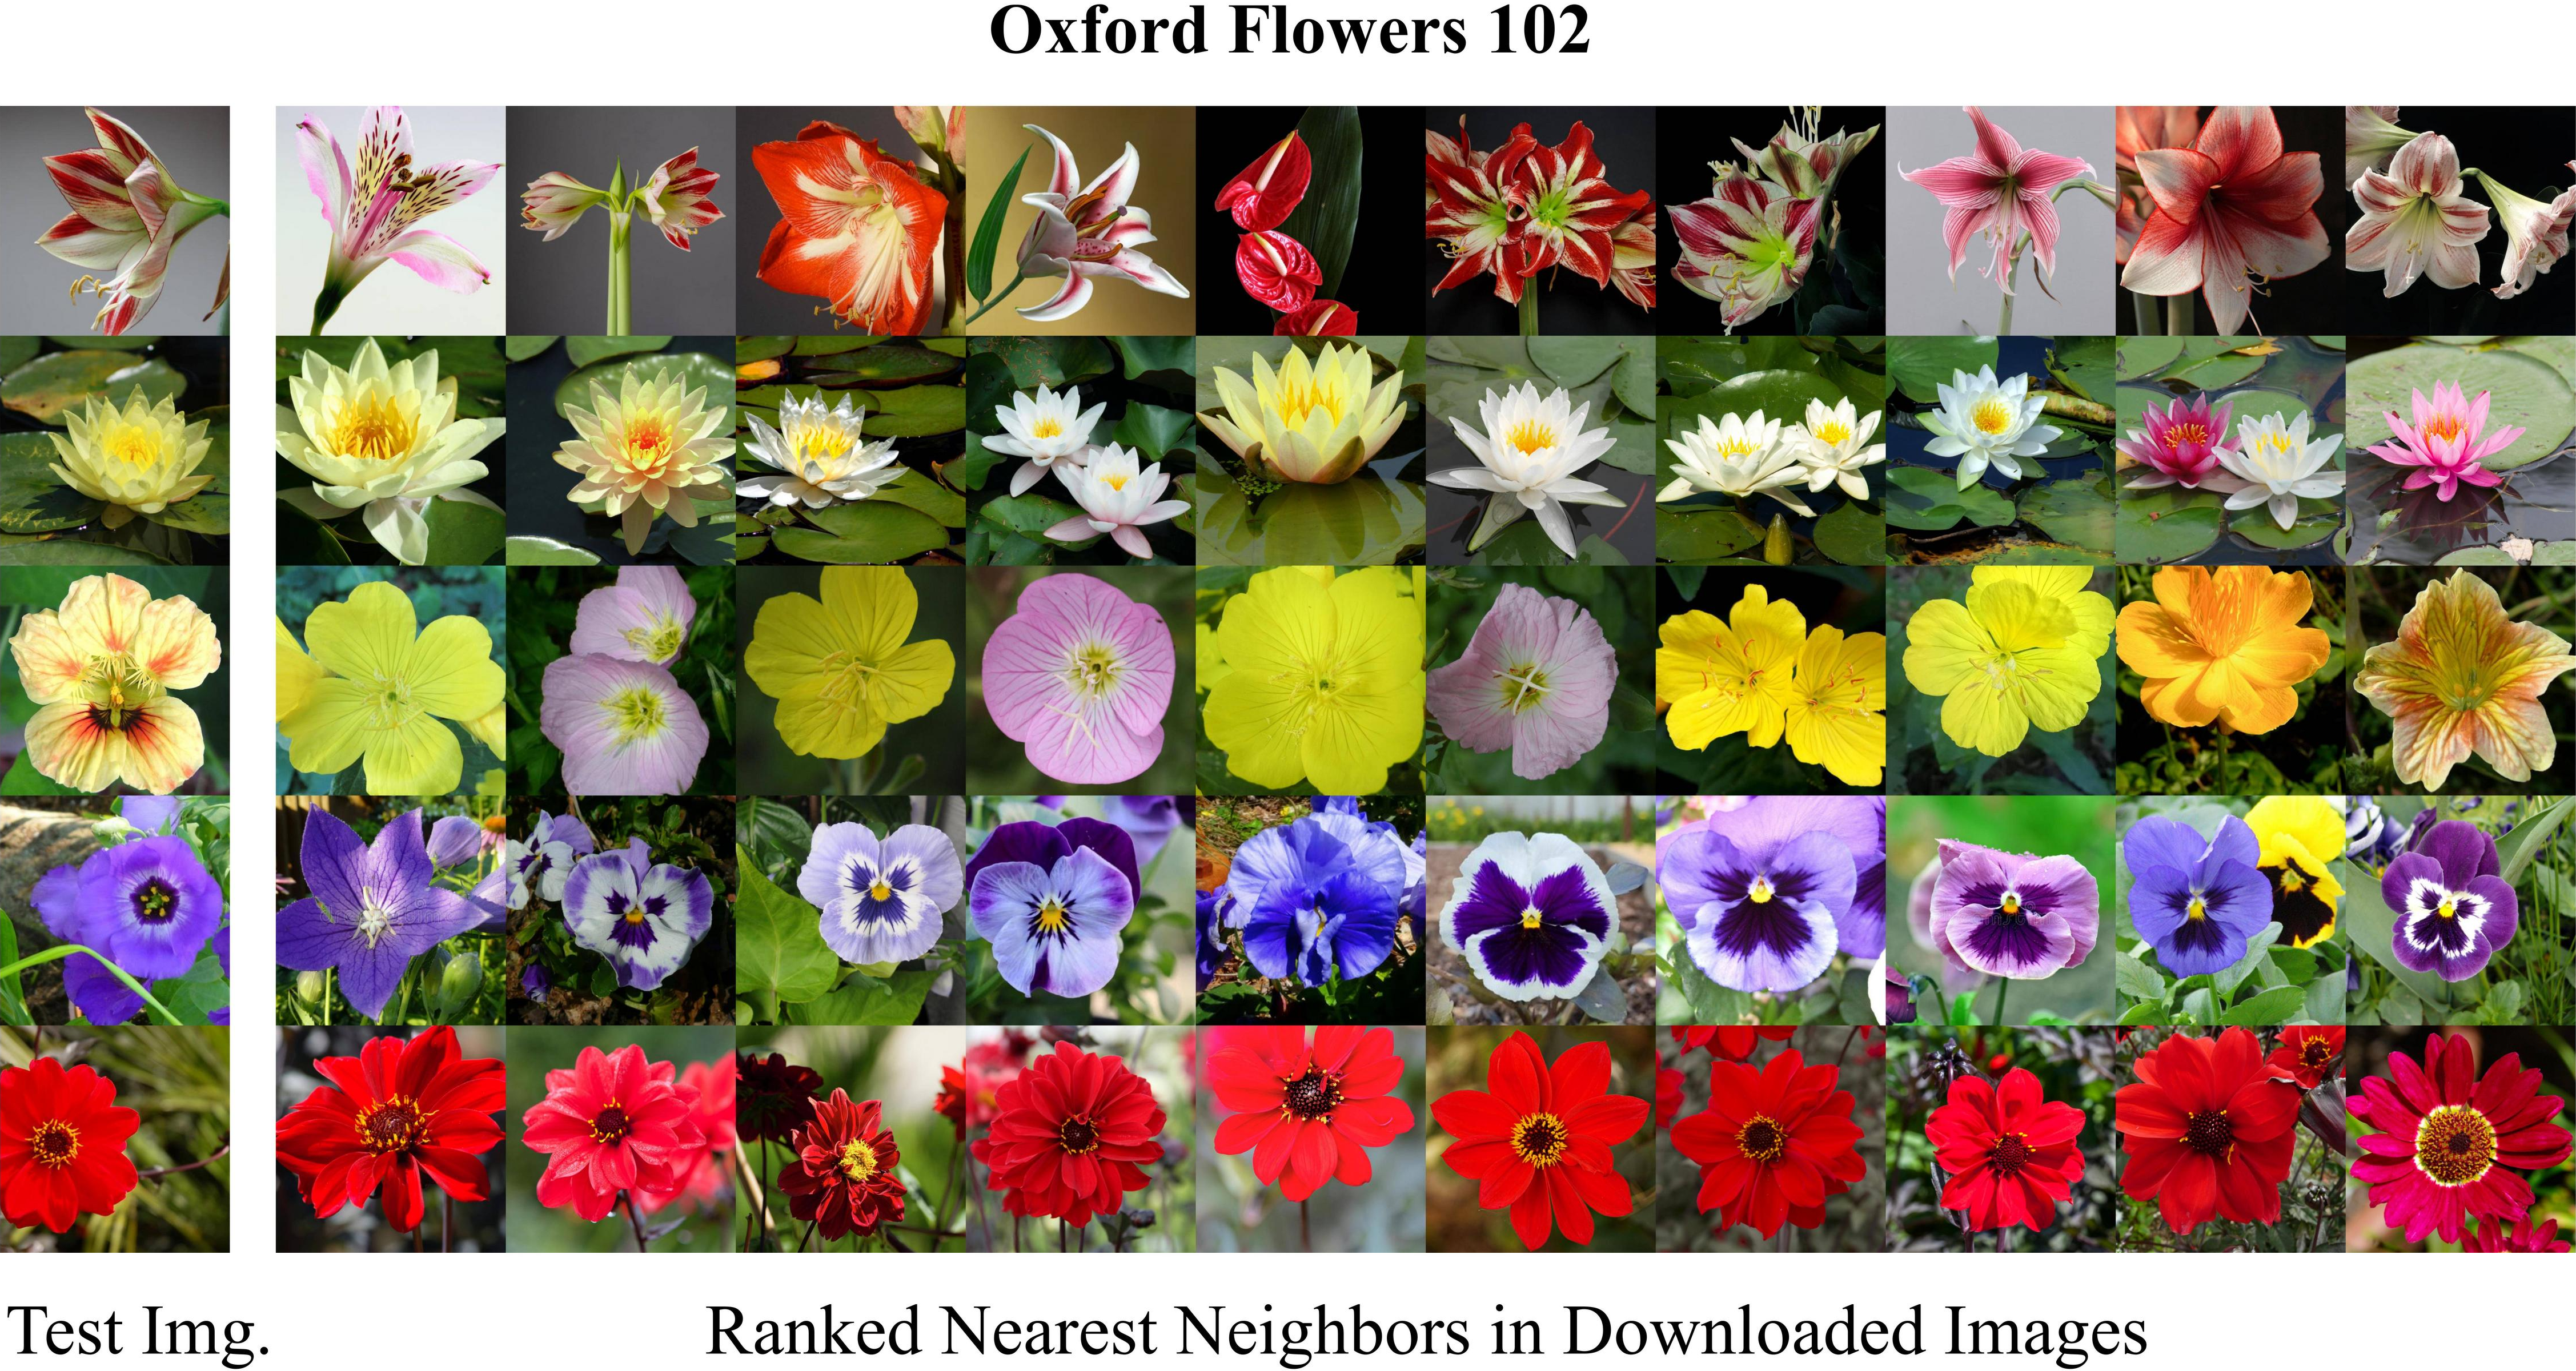
\includegraphics[width=0.75\textwidth]{figures/internet-nns/flowers.png}
        % \caption{Flowers}
        % \label{fig:flowers}
    \end{subfigure}
    \vspace{0.1em}

    \begin{subfigure}{\textwidth}
        \centering
        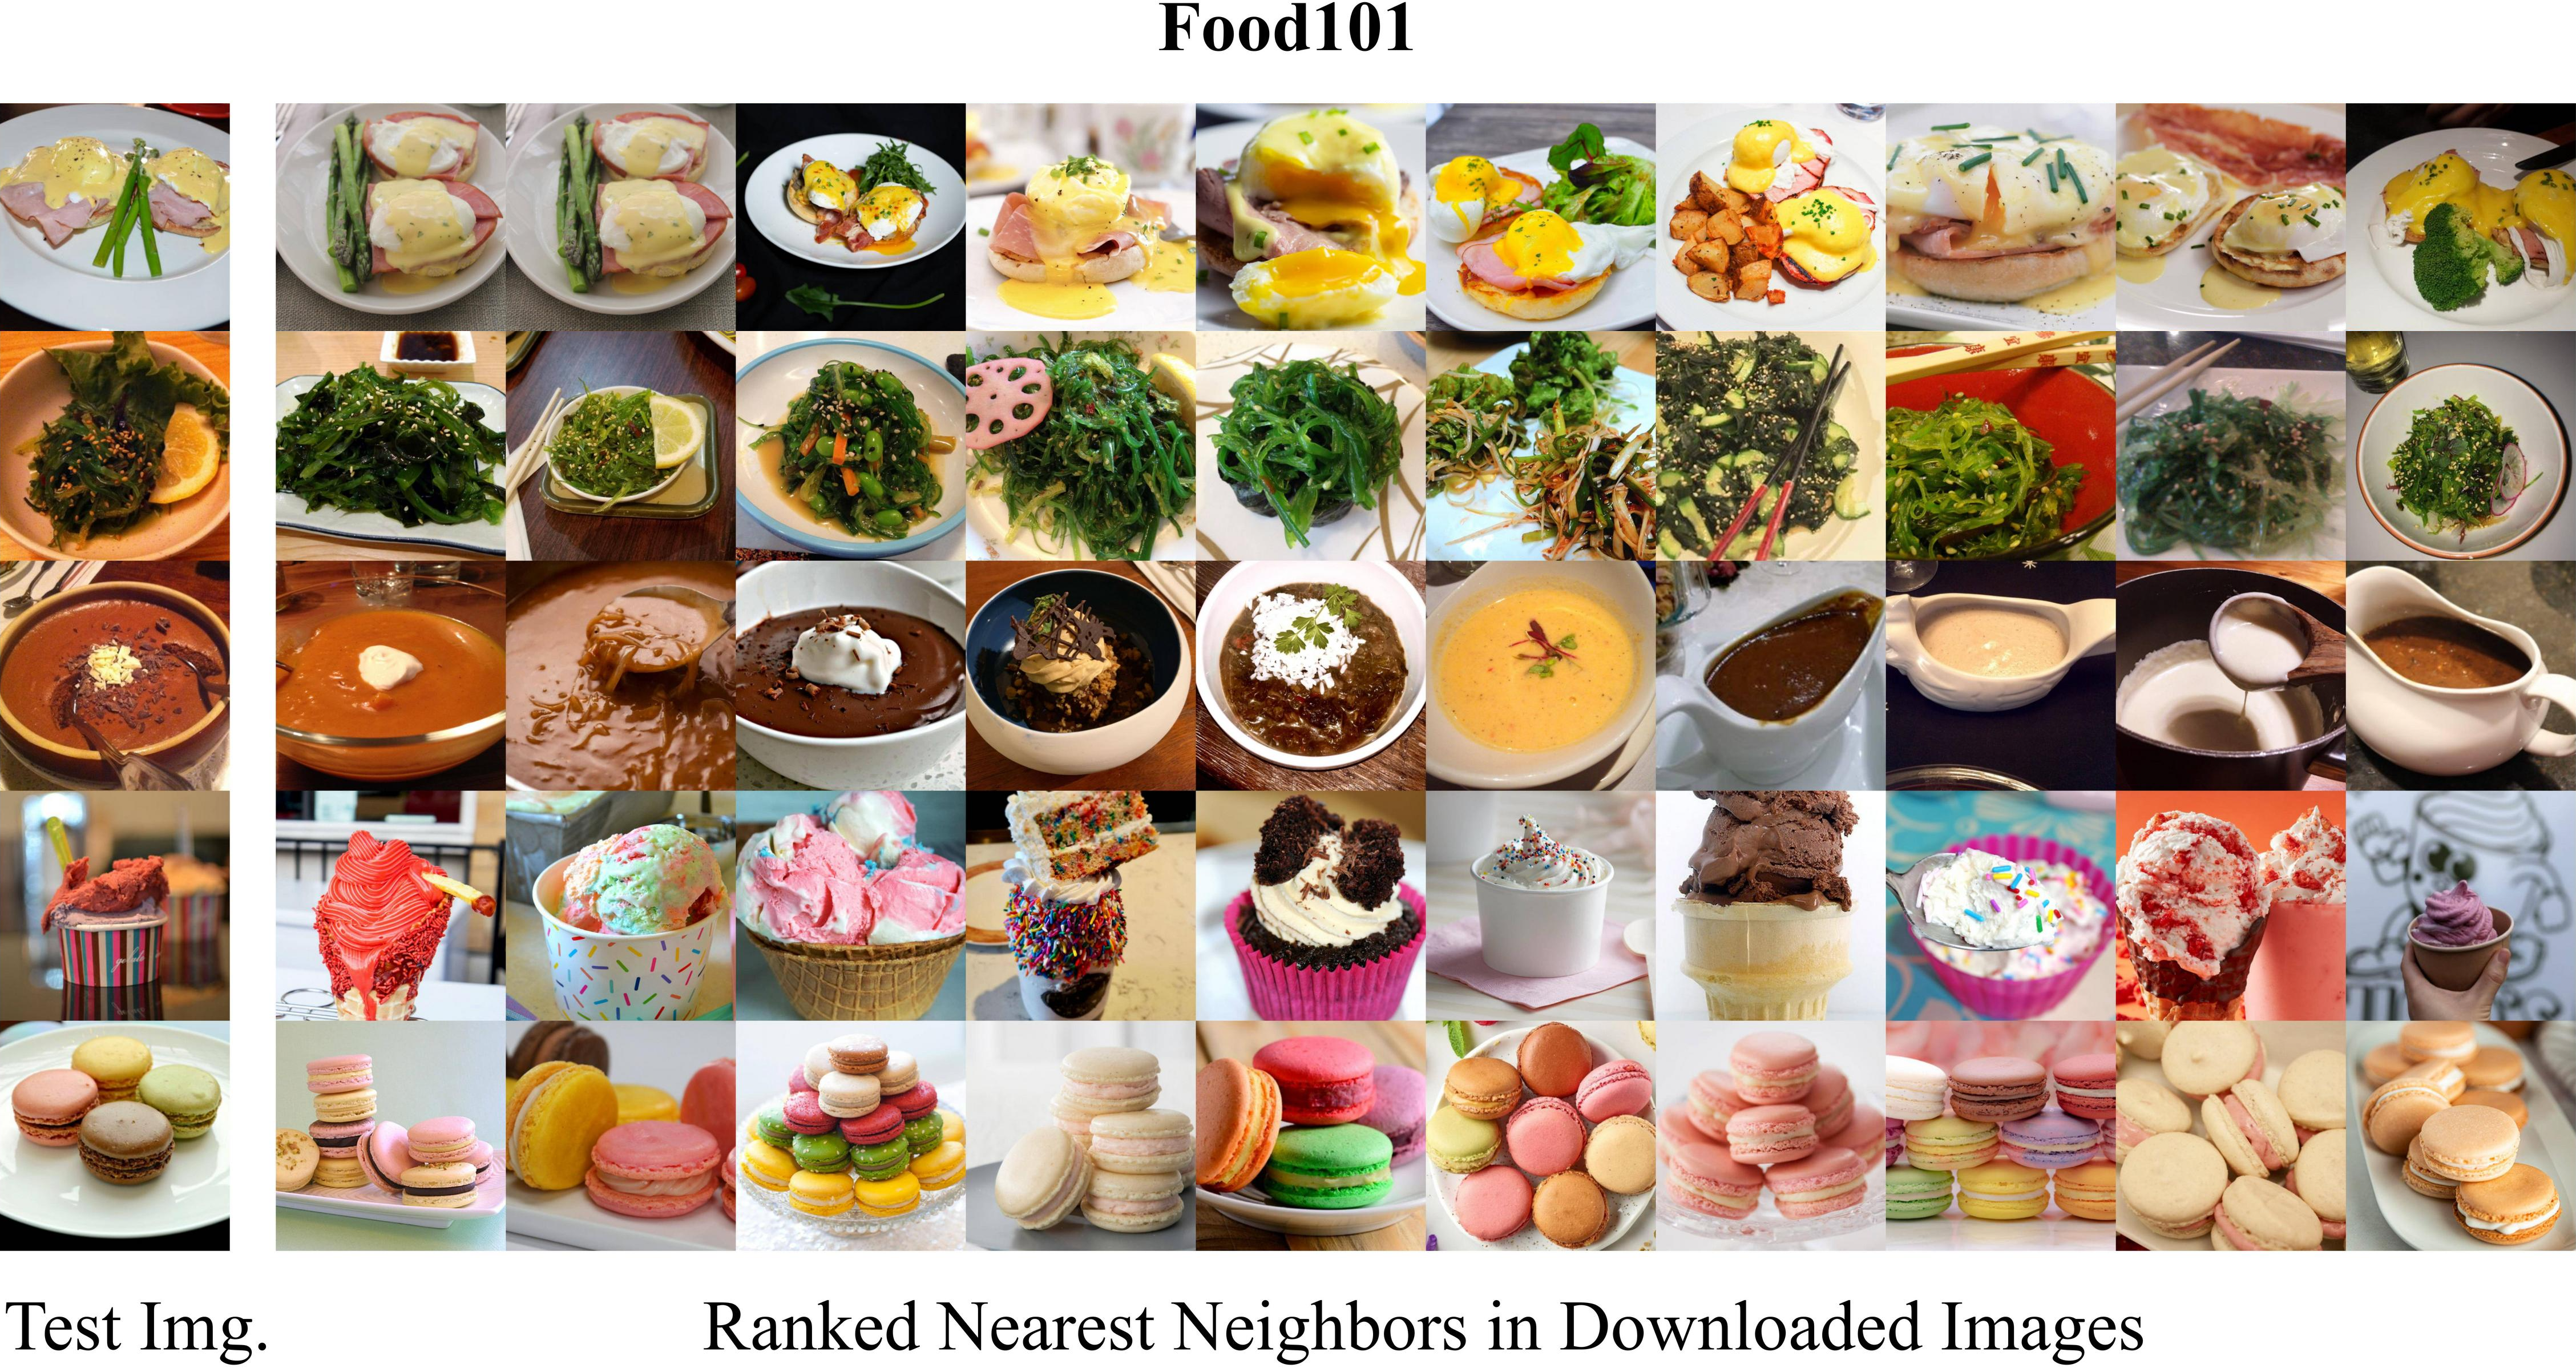
\includegraphics[width=0.75\textwidth]{figures/internet-nns/food.png}
        % \caption{Food}
        % \label{fig:food}
    \end{subfigure}
    \vspace{0.1em}

    \begin{subfigure}{\textwidth}
        \centering
        \includegraphics[width=0.75\textwidth]{figures/internet-nns/pets.png}
        % \caption{Pets}
        % \label{fig:pets}
    \end{subfigure}
    \vspace{0.1em}
    
    \caption{
        \textbf{Top-10 most similar online images}.
        The left column shows randomly chosen test set images from each dataset, and the right block shows the 10 most similar images in the downloaded data for each test image,
        ranked left to right.
        % ranked left to right in decreasing order of similarity and deduplicated (relative to other downloaded images, not the test images).
    }
    \label{fig:online_images}
\end{figure}

\subsection{Effect of image reward type}
\label{subsec:reward_analysis}
We run an ablation on the type of image relevance reward. Instead of calculating the image reward based on the average similarity to the $k=15$ nearest neighbors in representation space (as in \cref{subsec:ssl}), we also try using $k=1$ or the MoCo contrastive loss as the reward. Table~\ref{tab:image_reward} compares these three metrics in the label set-guided setting and shows that $k=15$ does best. We explain this result by qualitatively comparing the behavior of various metrics on Food101 in \cref{fig:reward_ranking} in the appendix. The MoCo loss does not identify relevant concepts, instead preferring images that are difficult to align across augmentations. Representation similarity with $k=1$ also fails, as it prefers images of zebras and text because these images are highly similar to a few outlier images in Food101. Our proposed reward with $k=15$ eliminates the influence of outliers and avoids this problem.

\begin{table}[h]
    \centering
    \begin{tabular}{lcc}
        \toprule
        Reward Type & Food \\
        \midrule
        MoCo loss & 81.2 \\
        1-NN sim  & 83.2 \\
        15-NN sim (ours) & \textbf{84.6} \\
        \bottomrule
    \end{tabular}
    \caption{\textbf{Ablation on type of image reward.}
    % We compare LP accuracy of 3 different rewards on Food in the label set-guided setting.
    MoCo loss does not identify relevant concepts, and $k=1$ similarity is too noisy to identify useful concepts. }
    \label{tab:image_reward}
\end{table}

\begin{figure}[h]
    \centering
    \includegraphics[width=0.5\linewidth]{figures/reward_ranking.pdf}
    % \vspace{-0.25in}
    \caption{\textbf{Top images preferred by different rewards.} We show the top 5 downloaded images ranked by 3 possible image rewards on the Food dataset. 15-NN (ours) prefers a variety of food images, whereas MoCo prefers noisy images out of the training distribution. 1-NN is thrown off by outliers in the Food dataset and thus prefers black images, text, and zebras.}
    \label{fig:reward_ranking}
    % \vspace{-0.06in}
\end{figure}

\subsection{Self-supervised Exploration Behavior on Other Datasets} 
\label{sec:progression_continued}
Just as \cref{fig:progression} in \cref{sec:exploration_behavior} showed how Internet Explorer progressively discovers useful data when targeting the Pets dataset, \cref{fig:birdsnap_progression}, \cref{fig:flowers_progression}, \cref{fig:food_progression}, and \cref{fig:voc_progression} show the progression of downloaded images when targeting Birdsnap, Flowers, Food, and VOC 2007 respectively. Note that this analysis is in the self-supervised setting, without any knowledge of the label set. 

\begin{figure*}
    \centering
    \includegraphics{figures/birdsnap_targets.pdf} \\
    \vspace{-0.8em}
    \includegraphics{figures/birdsnap-progression-1146-2col.pdf}
    \caption{\textbf{Progression of downloaded Birdsnap images.} This corresponds to Ours++ without using label set information. }
    \label{fig:birdsnap_progression}
\end{figure*}

\begin{figure*}
    \centering
    \includegraphics{figures/flowers_targets.pdf} \\
    \vspace{-0.8em}
    \includegraphics{figures/flowers-progression-1150-2col.pdf}
    \caption{\textbf{Progression of downloaded Flowers images.} This corresponds to Ours++ without using label set information. }
    \label{fig:flowers_progression}
\end{figure*}

\begin{figure*}
    \centering
    \includegraphics{figures/food_targets.pdf} \\
    \vspace{-0.8em}
    \includegraphics{figures/food-progression-1148-2col.pdf}
    \caption{\textbf{Progression of downloaded Food images.} This corresponds to Ours++ without using label set information. }
    \label{fig:food_progression}
\end{figure*}

\begin{figure*}
    \centering
    \includegraphics{figures/voc_targets.pdf} \\
    \vspace{-0.8em}
    \includegraphics{figures/voc-progression-1156-2col.pdf}
    \caption{\textbf{Progression of downloaded VOC2007 images.} This corresponds to Ours++ without using label set information. }
    \label{fig:voc_progression}
\end{figure*}



%%% Local Variables:
%%% coding: utf-8
%%% mode: latex
%%% TeX-engine: xetex
%%% TeX-master: "../thesis"
%%% End:
